% 1992 年上海卷第 11 题：四个函数图象选项（A）～（D）
% 每图均为 y=a^x 与 y=(a-1)x^2 的搭配；依固定扫描页重绘，只画拓扑与标号，不按比例
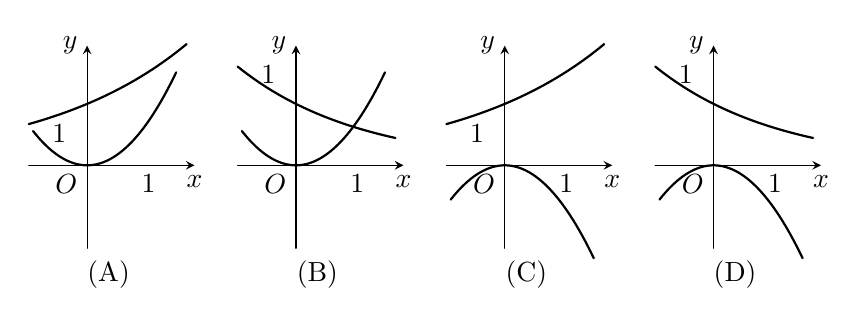
\begin{tikzpicture}[>=stealth,scale=0.78,line cap=round]
  % (A) 指数递增 + 抛物线开口向上
  \begin{scope}
    \draw[->] (-0.95,0)--(1.75,0) node[below] {$x$};
    \draw[->] (0,-1.35)--(0,1.95) node[left] {$y$};
    \node[below left] at (0,0) {$O$};
    \node[below] at (1,0) {$1$};
    \node[below left=4pt] at (0,1) {$1$};
    \draw[thick,domain=-0.95:1.62,samples=60] plot (\x,{exp(0.42*\x)});
    \draw[thick,domain=-0.88:1.45,samples=50] plot (\x,{0.72*\x*\x});
    \node at (0.35,-1.78) {(A)};
  \end{scope}
  % (B) 指数递减 + 抛物线开口向上
  \begin{scope}[xshift=3.4cm]
    \draw[->] (-0.95,0)--(1.75,0) node[below] {$x$};
    \draw[->] (0,-1.35)--(0,1.95) node[left] {$y$};
    \node[below left] at (0,0) {$O$};
    \node[below] at (1,0) {$1$};
    \node[above left=4pt] at (0,1) {$1$};
    \draw[thick,domain=-0.95:1.62,samples=60] plot (\x,{exp(-0.50*\x)});
    \draw[thick,domain=-0.88:1.45,samples=50] plot (\x,{0.72*\x*\x});
    \node at (0.35,-1.78) {(B)};
  \end{scope}
  % (C) 指数递增 + 抛物线开口向下
  \begin{scope}[xshift=6.8cm]
    \draw[->] (-0.95,0)--(1.75,0) node[below] {$x$};
    \draw[->] (0,-1.35)--(0,1.95) node[left] {$y$};
    \node[below left] at (0,0) {$O$};
    \node[below] at (1,0) {$1$};
    \node[below left=4pt] at (0,1) {$1$};
    \draw[thick,domain=-0.95:1.62,samples=60] plot (\x,{exp(0.42*\x)});
    \draw[thick,domain=-0.88:1.45,samples=50] plot (\x,{-0.72*\x*\x});
    \node at (0.35,-1.78) {(C)};
  \end{scope}
  % (D) 指数递减 + 抛物线开口向下
  \begin{scope}[xshift=10.2cm]
    \draw[->] (-0.95,0)--(1.75,0) node[below] {$x$};
    \draw[->] (0,-1.35)--(0,1.95) node[left] {$y$};
    \node[below left] at (0,0) {$O$};
    \node[below] at (1,0) {$1$};
    \node[above left=4pt] at (0,1) {$1$};
    \draw[thick,domain=-0.95:1.62,samples=60] plot (\x,{exp(-0.50*\x)});
    \draw[thick,domain=-0.88:1.45,samples=50] plot (\x,{-0.72*\x*\x});
    \node at (0.35,-1.78) {(D)};
  \end{scope}
\end{tikzpicture}
